\documentclass[12pt]{article}
\usepackage[utf8]{inputenc}
\usepackage[left=1in,right=1in,top=1in,bottom=1in]{geometry}
\usepackage{amsmath, amsfonts, amssymb, amsthm}
\usepackage{indentfirst}
\usepackage{graphicx}
\usepackage{textcomp}
\usepackage{hyperref}

\title{\Large
\includegraphics[height=3cm]{pics/UVM.png} \\
    CS253A QR: Reinforcement Learning\\
    Assignment \textnumero 8: n-step SARSA}
\author{Ayat Ospanov}
\date{\today}

\begin{document}
    \maketitle

    The experiment was held for n = \{1, 2, 3, 4, 5, 6\}. The results are given
    in \autoref{fig:orig} and \autoref{fig:smooth}. From the original graph
    it is barely visible which is better and which is not. But we can see that
    there exponential curves, e.g. n=2. So lets approximate this lines with
    polynomials of 2nd degree. Doing this we get \autoref{fig:smooth}. It is
    now easily distinguishable which n is best for Pacman. At least for the scope
    we have, i.e. for 10000 iterations.

    Having n=\{3, 4\} has high constant convergence rate, while n=\{5, 6\} is
    slightly worse. n=1 is the worst case and converges very slow. For n=2 we
    can see exponential convergence (it is a bowl shape because we approximated
    it with the polynomial, not exponential function) and in long term it will
    converge the fastest. So n = 2 is the best.

    \begin{figure}[!t]
        \centering
        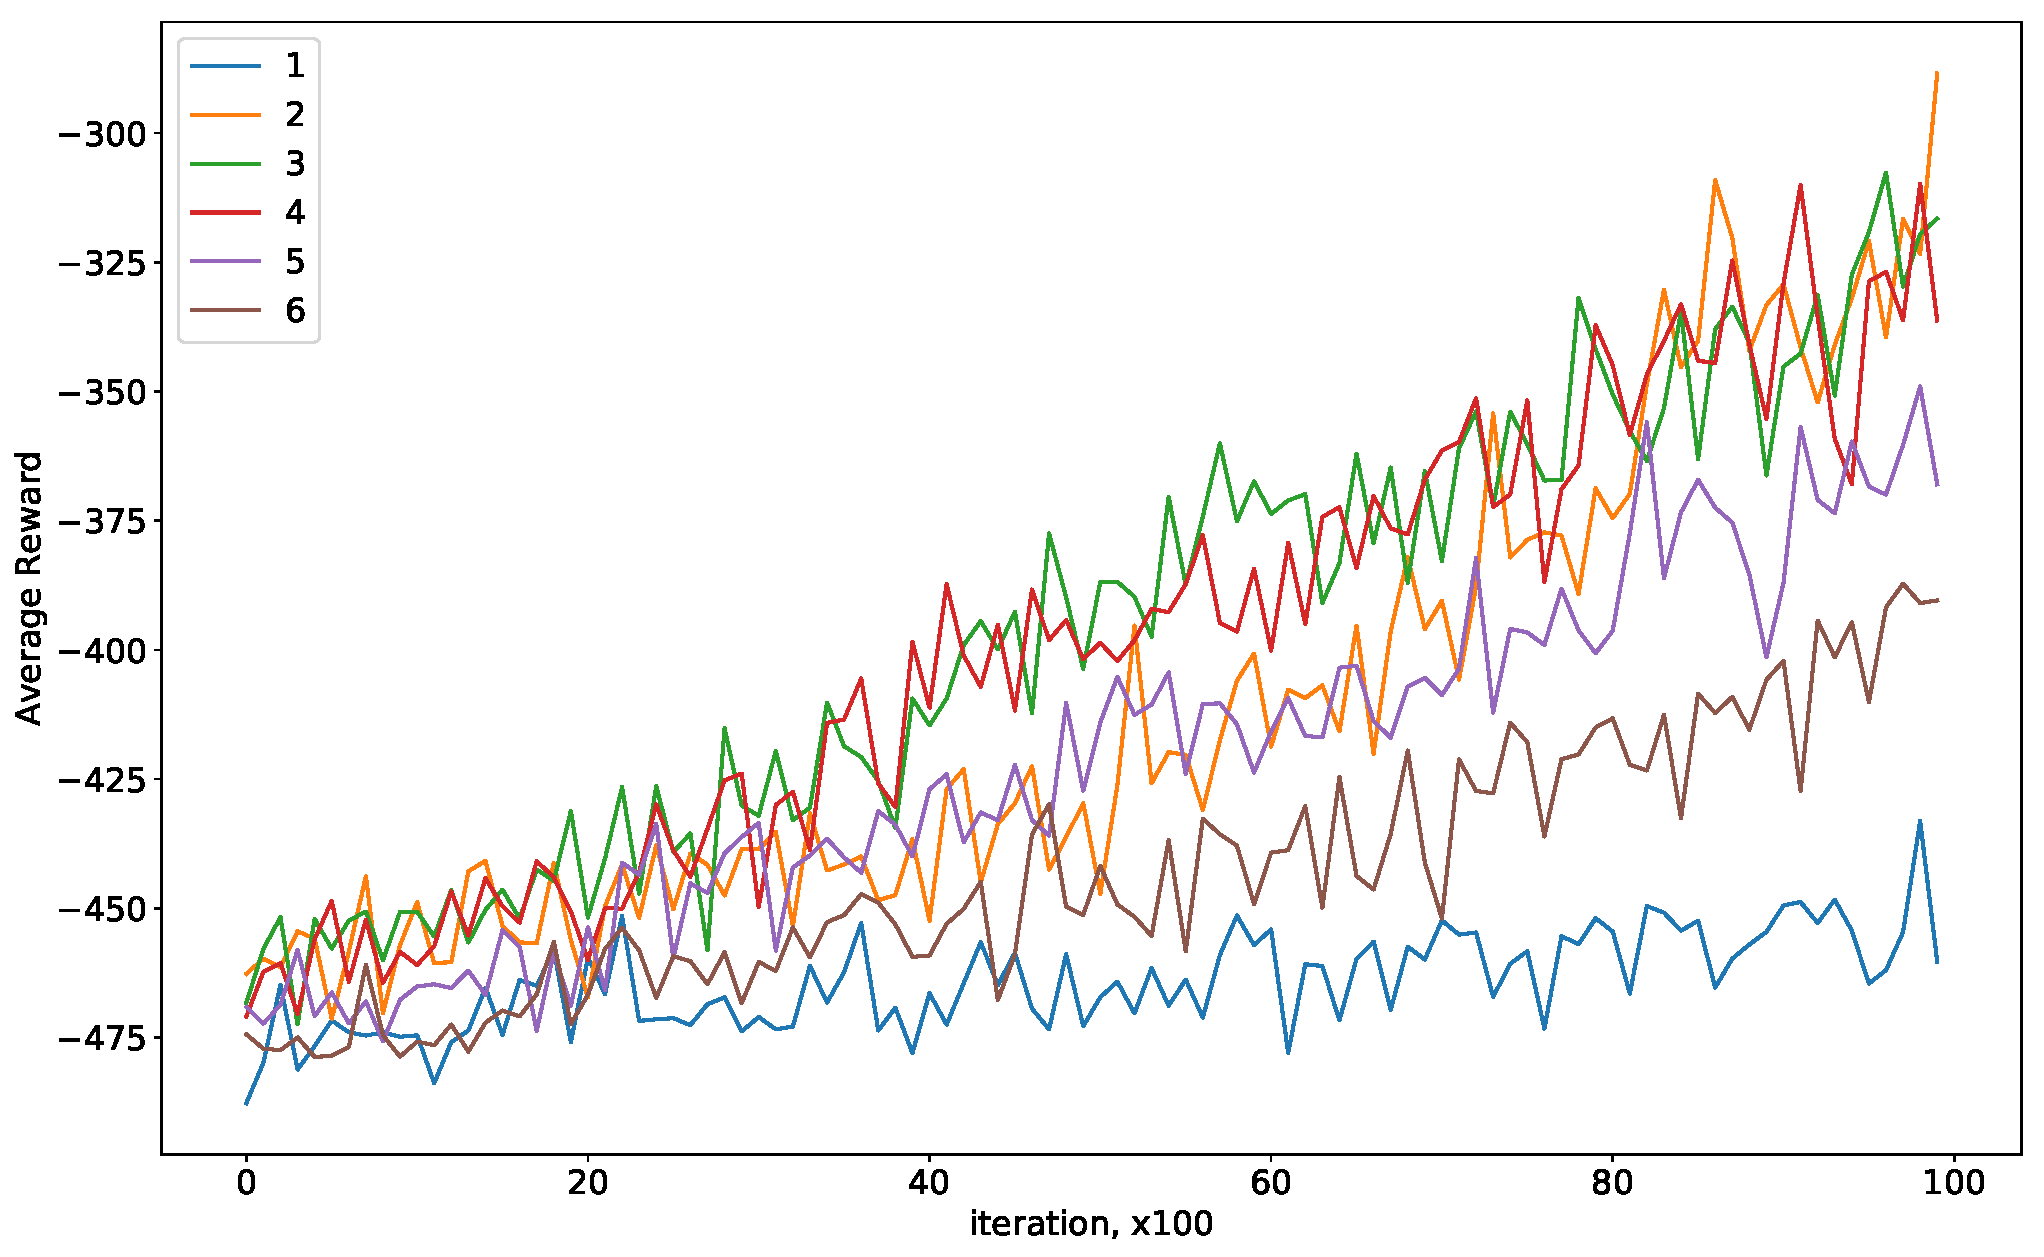
\includegraphics[width=\linewidth]{pics/graph}
        \caption{Average reward for 10000 iterations over 10 runs}
        \label{fig:orig}
    \end{figure}

    \begin{figure}[!t]
        \centering
        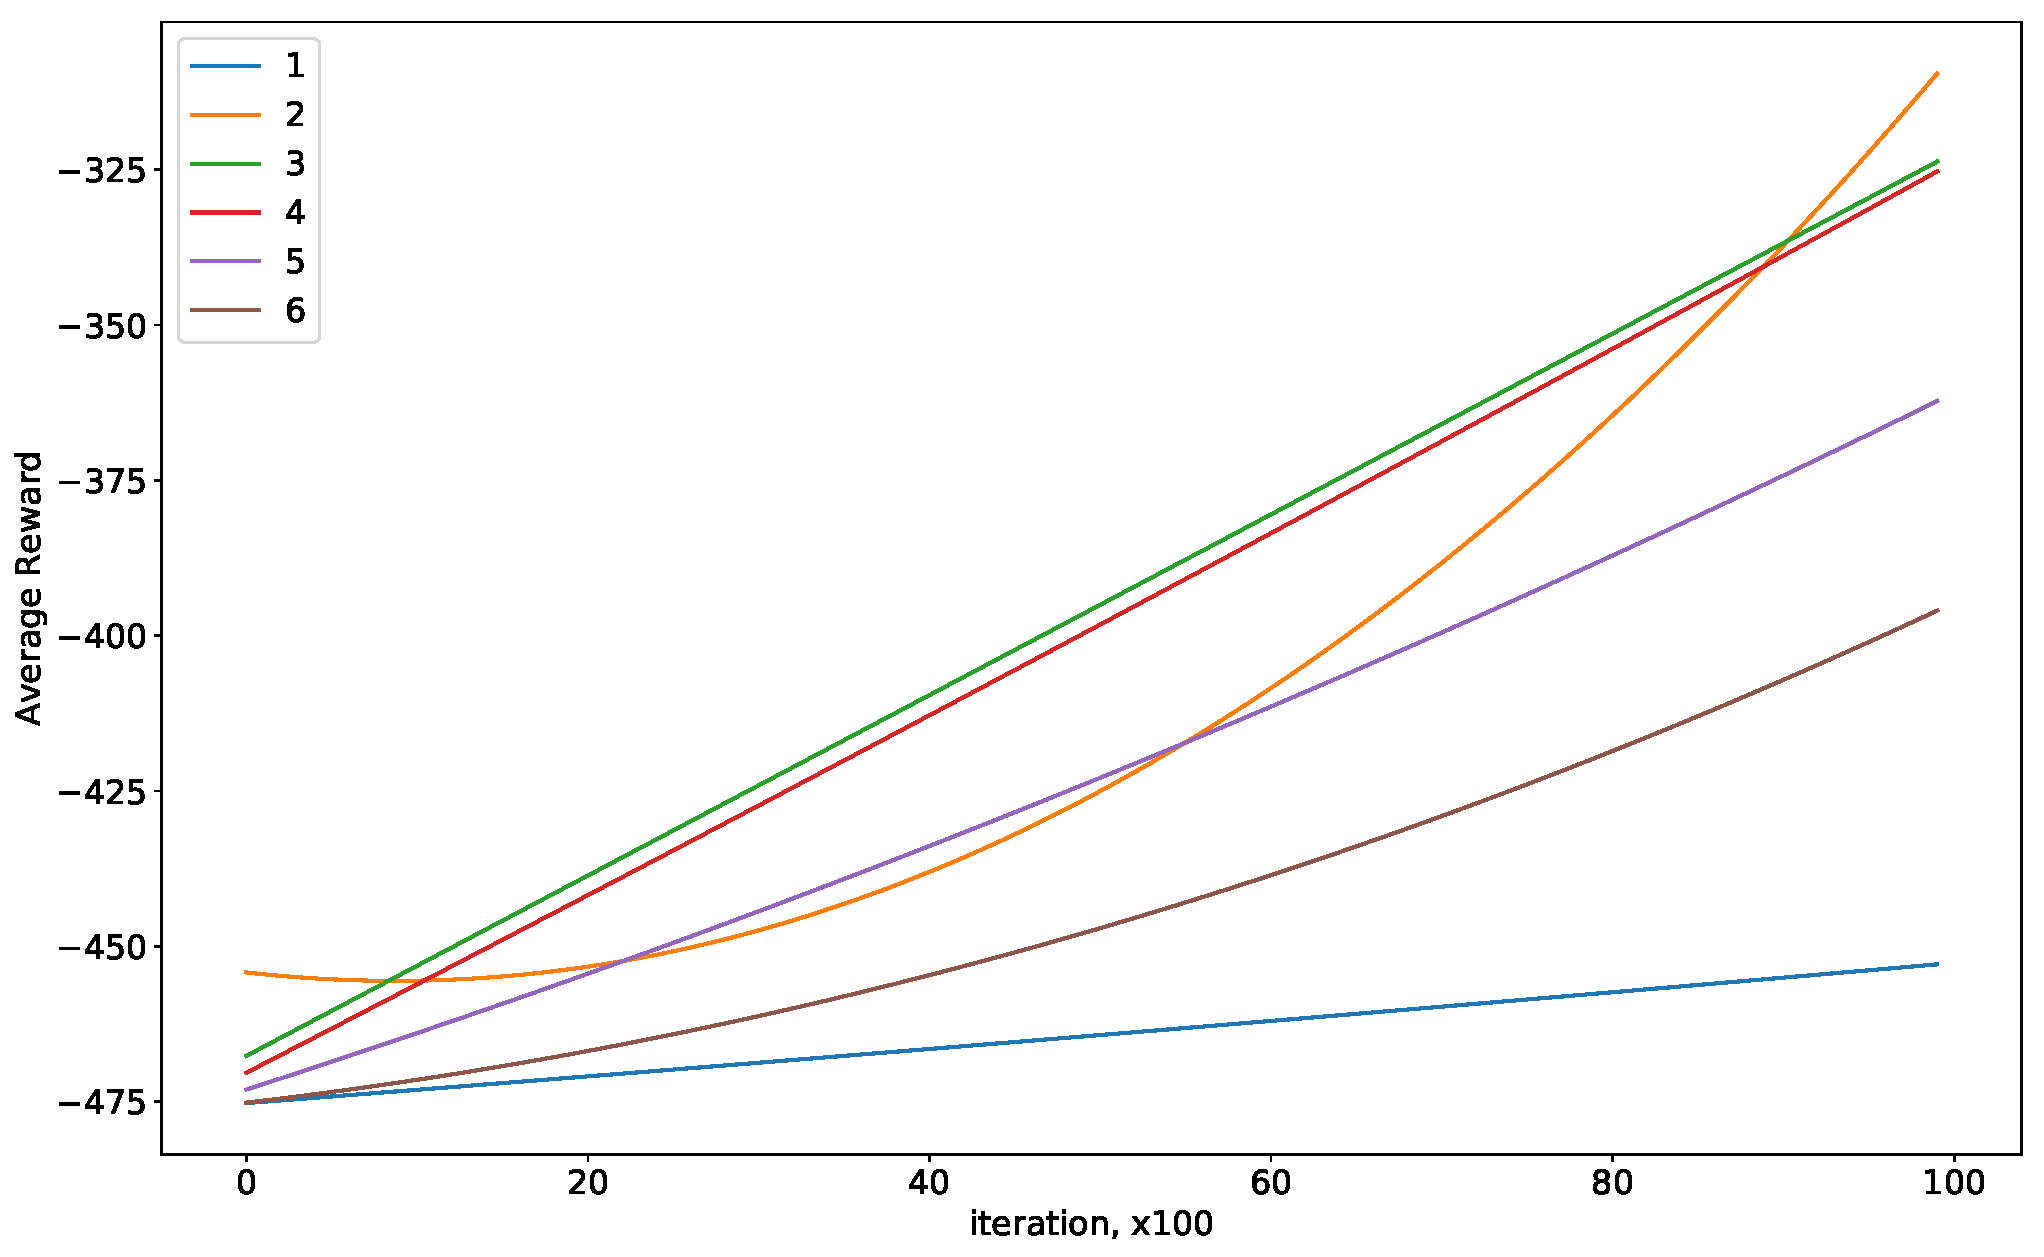
\includegraphics[width=\linewidth]{pics/graph_smooth}
        \caption{Smoothed average reward for 10000 iterations over 10 runs}
        \label{fig:smooth}
    \end{figure}

\end{document}
